 %!TEX program = latexmk
\documentclass[12pt,fleqn]{article}
\usepackage{setspace}
\usepackage{float}

\usepackage[english]{babel}
\PassOptionsToPackage{table,xcdraw}{xcolor}
\usepackage[notransparent]{svg}
% \usepackage[utf8x]{inputenc}

\usepackage[style=apa, backend=biber]{biblatex}
\addbibresource{references.bib}

% A few common packages
\usepackage{amsmath}
\usepackage{amssymb}
\usepackage{amsthm}
\usepackage{array}
\usepackage{graphicx}
\usepackage{relsize}
\usepackage[titletoc]{appendix}
\usepackage{caption}
\captionsetup[table]{skip=10pt plus 0.01pt}
\usepackage{subcaption}  % \begin{subfigure}...\end{subfigure} within figure
\usepackage{multirow}
\usepackage{tabularx}
\usepackage{makecell}
\usepackage{booktabs}
\usepackage{ltablex}
\usepackage[autostyle, english = american]{csquotes}



% Uncomment the following to attempt to enforce Type 1 or TrueType 
% fonts. ProQuest does not want the type 3 fonts used by default as
% of Dec. 2019 - see 
% https://support.proquest.com/articledetail?id=kA01W000000k9o2SAA . 
% If you are unable to embed fonts such as 'Zapf Dingbats' or 
% 'Symbol', try using raster images (.jpg or .png) instead of vector 
%images (.pdf or .eps).
% \usepackage[T1]{fontenc} 

% plainpages=false fixes the "duplicate ignored" error with page counters
% Set pdfborder to 0 0 0 to disable colored borders around PDF hyperlinks
\usepackage[plainpages=false,pdfborder={0 0 0}]{hyperref}

\begin{document}

\title{Modeling Decanalization with Homeostatic Reinforcement Learning}
\author{Joshua Clingo and Jeff Yoshimi}
\maketitle
µ
\begin{abstract}
Living organisms continuously manage their homeostatic setpoints but sometimes fall into the ruts and grooves of an entrenched or canalized behavioral repertoire. This manifests in a wide variety of ways, from overconsumption of scarce resources to repetitive unhealthy behavior, in cases of depression or anxiety. Clinicians are increasingly employing interventions, from psychoactive drugs to targeted stimulus regimes, to transiently decanalize entrenched behaviors and recanalize them into more adaptive patterns. These metaphors are long-standing, but have not been formally studied in explicit computational models. We present the first such model to our knowledge, a computational model of canalization, decanalization, and recanalization in a homeostatic navigation task. We compared homeostatic reinforcement learning (HRL) with a negative feedback (NF) reward function under matched canalization and decanalization conditions. In this setting, HRL agents showed improved post-decanalization homeostatic performance, relative to matched no-decanalization controls, whereas NF agents did not. We offer the model as a formal instantiation of a candidate mechanism by which temporary destabilization can produce more optimal behaviors in a constrained environment.
\end{abstract}

% !TEX root = ./main.tex
\section{Introduction}

Organisms are constantly confronted with the trade-off between the pursuit of known sources of reward (exploitation) and uncertain sources of reward (exploration) \parencite{stephens_foraging_1986}. Although organisms ideally switch between exploration and exploitation at will and at optimal times \parencite{pearson_decision_2014}, they often either remain in one of those modes for too long or continue to cycle between them in non-optimal ways \parencite{barack_neurocomputational_2016, addicott_primer_2017}. This can lead to habituated behavior patterns that are in conflict with their homeostatic needs \parencite{bernard_lectures_1974}. From a dynamical systems perspective, organisms get stuck in the wells of a fixed set of attractors—in the ruts and grooves of a ‘canalized’ landscape of behaviors \parencite{waddington_canalization_1959, carhart-harris_canalization_2023}. From a Bayesian perspective, belief updating shifts from a flexible, dynamic process to a fixed process, leading to repeated suboptimal behaviors \parencite{harle_anhedonia_2017} and rigid response patterns. From a reinforcement learning perspective \parencite{sutton_reinforcement_1998}, the interaction of meta-parameters and environmental factors leads to reduced exploration and therefore over-exploitation of rewarding resources \parencite{huys_mapping_2013}. These resources are discounted in perceived value, resulting in ‘observational overfitting’, where agents stop exploring altogether because they fixate on the wrong observational factors—resources that once were rewarding but are no longer rewarding \parencite{song_observational_2019}.

The problem of ‘hypercanalization’ (over-canalization) has been recognized in several areas of psychology, cognitive science \parencite{lloyd_understanding_2023}, clinical practice \parencite{addicott_primer_2017}, and in “integrative psychotherapy” \parencite{schiepek_self-organization_2014, schiepek_integrative_2015, schiepek_psychotherapy_2017}. With integrative psychotherapy, intentionally alternating between \emph{decanalization} and \emph{recanalization} is central to the therapeutic process, where these modal shifts allow for integration and re-integration of positive behavioral patterns. These theorists draw inspiration from dynamical systems theory (formerly ‘synergetics’ \parencite{haken_synergetics_1977}), focusing on how whole systems often exhibit emergent behaviors not predicted by their individual components. They also draw on control theory \parencite{wiener_cybernetics_2019} (or in the earlier literature, `cybernetics’), the study of systems with feedback loops, tracking how information is communicated and controlled within those systems, particularly in modeling mental health pathologies and devising solutions for them. In these integrative psychotherapeutic frameworks, dynamical systems theory can be used to model high-level behaviors that emerge from lower-level behaviors. Theoretical frameworks in this area include homeostatic setpoint management \parencite{keramati_homeostatic_2014} and allostasis \parencite{sterling_allostasis_1988, sterling_allostasis_2012}. In these, complex behaviors emerge and stabilize over time through effective reinforcement learning \parencite{keramati_homeostatic_2014} and through temporal discounting of positive rewards in anticipation of greater rewards and/or a reduction in uncertainty or future loss. However, the learning process can backfire if the organism is observationally overfitted, relying on rigid expectations for possible rewards in its environment.

In these frameworks, hypercanalized behaviors such as depression, anxiety, PTSD, addiction, and OCD are said to result from over-weighted priors—rigid and stubborn response patterns that canalize behavior toward a downward spiral of maladaptive, self-fulfilling, and self-destructive behavior \parencite{scheffer_dynamical_2024}. This framework has made its way to psychedelic-assisted psychotherapy, during which \cite{carhart-harris_entropic_2014}—among others \parencite{hipolito_pattern_2023, girn_complex_2023, juliani_deep_2024}—have proposed that psychedelics provide an entropic burst that destabilizes brain networks, leading to long-term psychological transformation. They propose that focused destabilization during the psychotherapeutic process can address many of the otherwise intractable conditions marked by behavioral canalization.

For the most part\footnote{One exception is the CANAL model—an extension of REBUS \parencite{carhart-harris_rebus_2019}—\cite{juliani_deep_2024} (\citeyear{juliani_deep_2024}), which proposes that there are two independent types of canalization at play in mental health pathologies, and it is the intersection of these that produces ‘sticky attractors’. Drawing on neural network theory, \parencite{barak_recurrent_2017}, they propose that canalization can describe both overfitting (inference) and plasticity loss (learning). Decanalization is the opposite of both, leading to temporary underfitting and increased metaplasticity.}, these ideas have remained metaphorical. Although prior conceptualizations and hypotheses we have described provide helpful conceptualizations, they fall short of actually modeling and directly confronting their assumptions. In the absence of any quantitative foundation, the overall value of these approaches is limited. To address this, we synthesized these ideas and developed a simulation that translates these assumptions into observable behavior. Our primary intention was to translate the assumptions of earlier conceptualizations into formal structures that can be quantified and compared—by doing so, we can hope to sharpen these conceptualizations, demonstrate their applicability to agentic behavior in simulated environments, and highlight open questions that reveal themselves once the nebulous cluster of informal ideas is pressed into direct service as a behavioral simulation. In this paper, we address this gap in the literature by developing a computational model of canalization and hypercanalization and showing how an agent in a simulated environment can improve its well-being by an appropriately administered set of decanalization events.

Our model of decanalization is inspired by a series of papers by Carhart-Harris and collaborators on the entropic brain \parencite{carhart-harris_entropic_2014,carhart-harris_entropic_2018} and canalization \parencite{carhart-harris_rebus_2019} in altered states induced by psychedelics, along with Hipólito et al.'s (\citeyear{hipolito_pattern_2023}) pattern-breaking model. We also rely on Juliani et al.'s “Deep CANALs” (\citeyear{juliani_deep_2024}), which asserts that the intersection of overfitting and low plasticity results in major depressive disorder, OCD, substance use disorder, and generalized anxiety disorder, which we treat as instances of hypercanalization. According to Juliani et al., decanalization acutely alters synaptic weights, sensory observations, and induces metaplasticity: “[Acute decanalization] is a function of both the current environmental context (made partially available to the model through a sequence of sensory observations) and the state of the system within the synaptic weight landscape. The inferred set of beliefs in a given instance are a function of the location of the system within the neural activity landscape.” To simulate this in our agent-based model, we represent sensory observations as observations about internal and external states. Synaptic weights correspond to a set of associations between states, actions, and rewards learned through reinforcement learning. Neural activity corresponds to short-term beliefs represented by the state variables of the solutions. Metaplasticity is represented by factors that influence the learning dynamics of the system.

To model decanalization and recanalization, we use homeostatic reinforcement learning. This approach involves movement, planning, and reward-seeking to minimize setpoint deviations across a range of homeostatic setpoints, ranging from basic biological needs to cognitive and emotional demands. An agent that is well-adapted to its environment should be able to effectively perform these fundamental actions. However, as we see with humans suffering from mental pathologies, even basic homeostatic regulation can break down when behavioral distortions occur. Instead, those inflicted with mental pathologies tend to hypercanalize around just a few sources of reward that produce results that are far from optimal. They struggle to adapt to new surroundings, preferring to repeat even minimally rewarding actions. Moreover, they discount possible alternative sources of reward. In short, they get stuck in canalized (entrenched) patterns. Our simulation captures these dynamics.

\section{Methods}

We built a simulation sandbox in Unreal Engine to directly explore canalization and decanalization dynamics. Entrenched behavioral patterns—often visualized as gravitational wells—were represented as variable-cost pathways through which an agent traversed a simulated world of homeostatic state-altering resources. Using reinforcement learning, the agent was trained to behave rationally, according to a set reward function, reducing the discrepancy between the outcome the model predicted and what was actually observed. In each training cycle, the agent observed a state, chose an action, and received a reward based on that action. We used a variation of the homeostatic reinforcement learning drive reduction formula as the primary reward function, contrasting it with negative feedback in the analysis.

The agent was modeled as a cube that moves forward at a constant velocity, while an internal homeostatic variable, $h_t$ (described below), decreased at a fixed rate. To increase $h_t$, cylindrical pellets that increased $h_t$ after overlap with the agent were distributed throughout the environment.  Repeated traversals of the same paths across the 2D surface of the environment were tracked by partitioning the environment into planar tiles that were associated with a memory of past visits, such that when the agent collided with them, there was reduction in $h_t$ proportional to the number of past visits. This penalized movement but penalized it less when familiar paths were taken. The arena was enclosed by a rectangular boundary. When the agent crossed this boundary, its position was wrapped\footnote{This design choice prevented edge effects that would otherwise require the agent to manage the boundary as an additional environmental factor and potentially introduce edge-induced artifacts into the behavioral data.} to the opposite side, resulting in a toroidal, arcade-style world.

To train the agent, we used proximal policy approximation (PPO), a model-free reinforcement learning method. PPO works by sampling many different behavioral trajectories (action-sequences) relative to the current policy, and tracking rewards obtained on each of these trajectories. When the trajectory terminates, an ‘advantage’ is calculated for every action taken on the corresponding trajectory (advantage corresponds to how much better or worse an action turned out compared to expectation). The policy is updated to increase the probability of actions with positive advantage and decrease the probability of actions with negative advantage. To keep learning stable and efficient, PPO constrains each update so that the new policy does not move too far from the old one. PPO tends to be relatively stable and effective in complex learning environments.

We used version 5.5 of Unreal Engine, a 3D computer graphics game engine that performs realistic physics simulation, rendering, and state management. To implement reinforcement learning, we used the ‘Learning Agents’ plugin. This plugin facilitates the transmission of configuration and state information to PyTorch, where the training process is conducted using PyTorch's implementation of PPO. Upon completion of the training phase, we loaded the trained model and subsequently observed and measured agent behavior in a variety of scenarios.

\begin{figure}
    \centering
    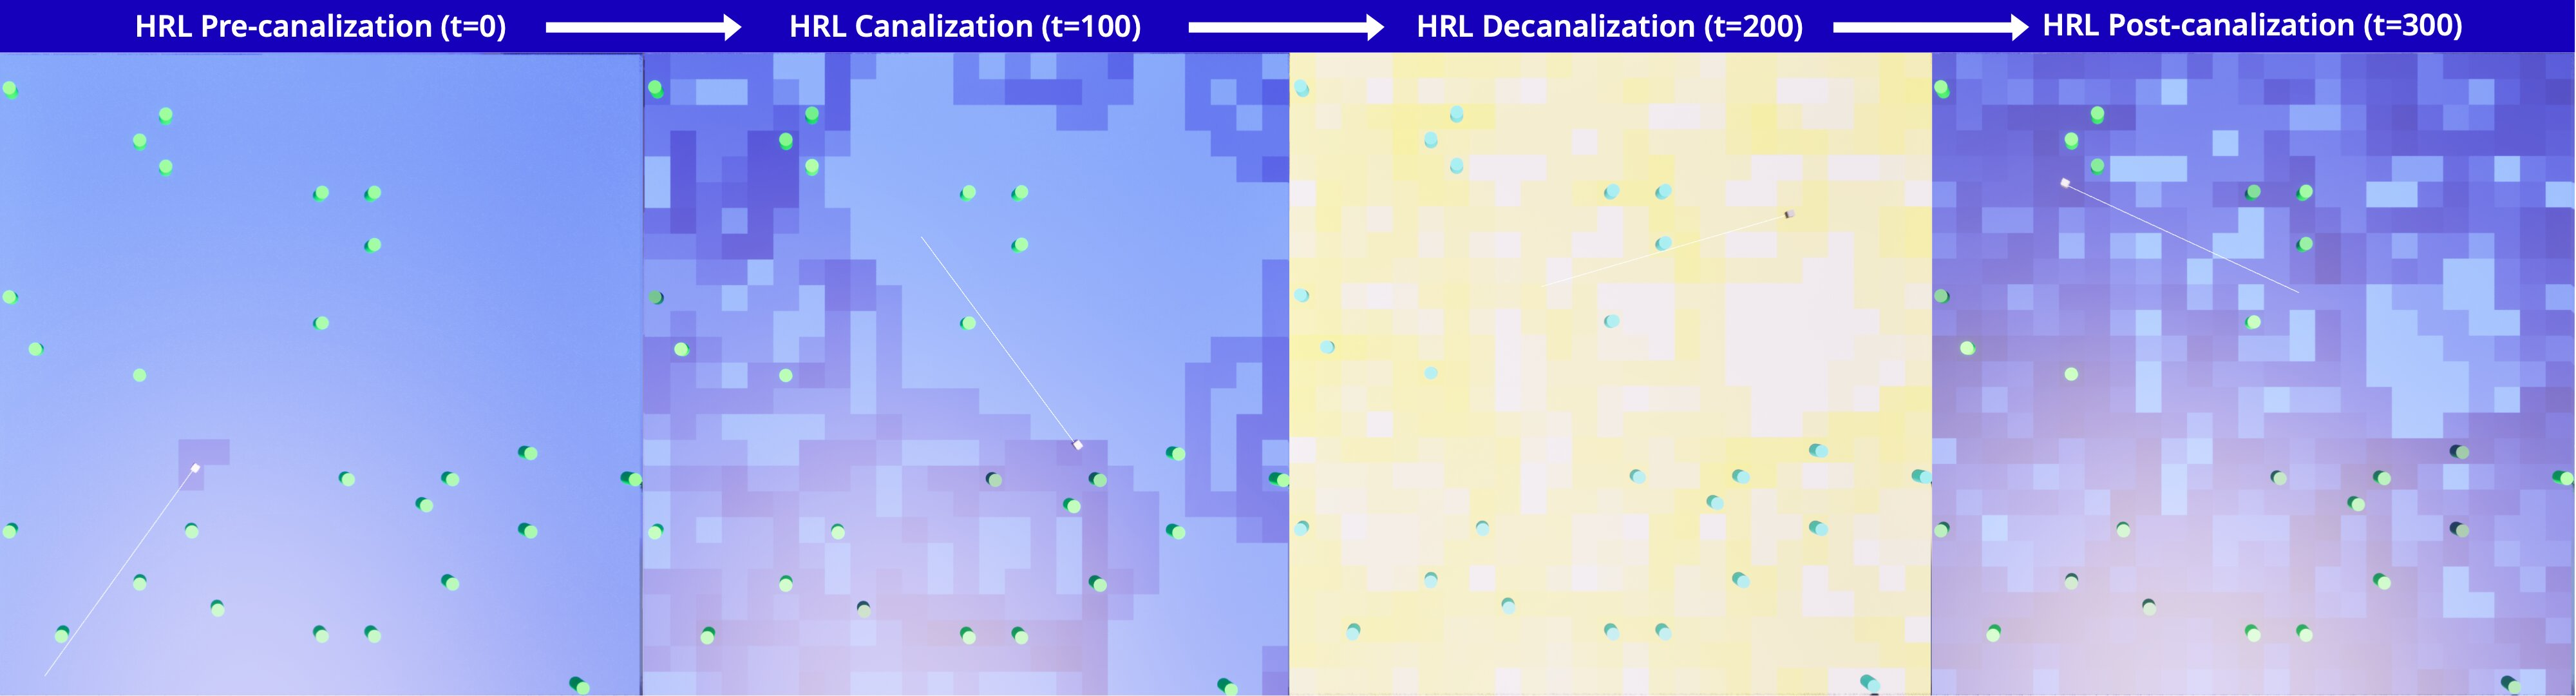
\includegraphics[width=1\linewidth]{./figures/canalization-phases.png}
    \caption{Each of the four panels corresponds to a top-down view of a trained agent. The small yellow square in each panel corresponds to the agent; the orientation of the agent and the vision raycast are represented by the white line. The four panels correspond to different canalization phases. The color of each tile represents its traversal cost. Pellets are in green and are shaded in proportion to how rewarding they are. The yellow panel indicates the decanalization phase and its altered perceptual properties.}
\end{figure}

\begin{figure}
    \centering
    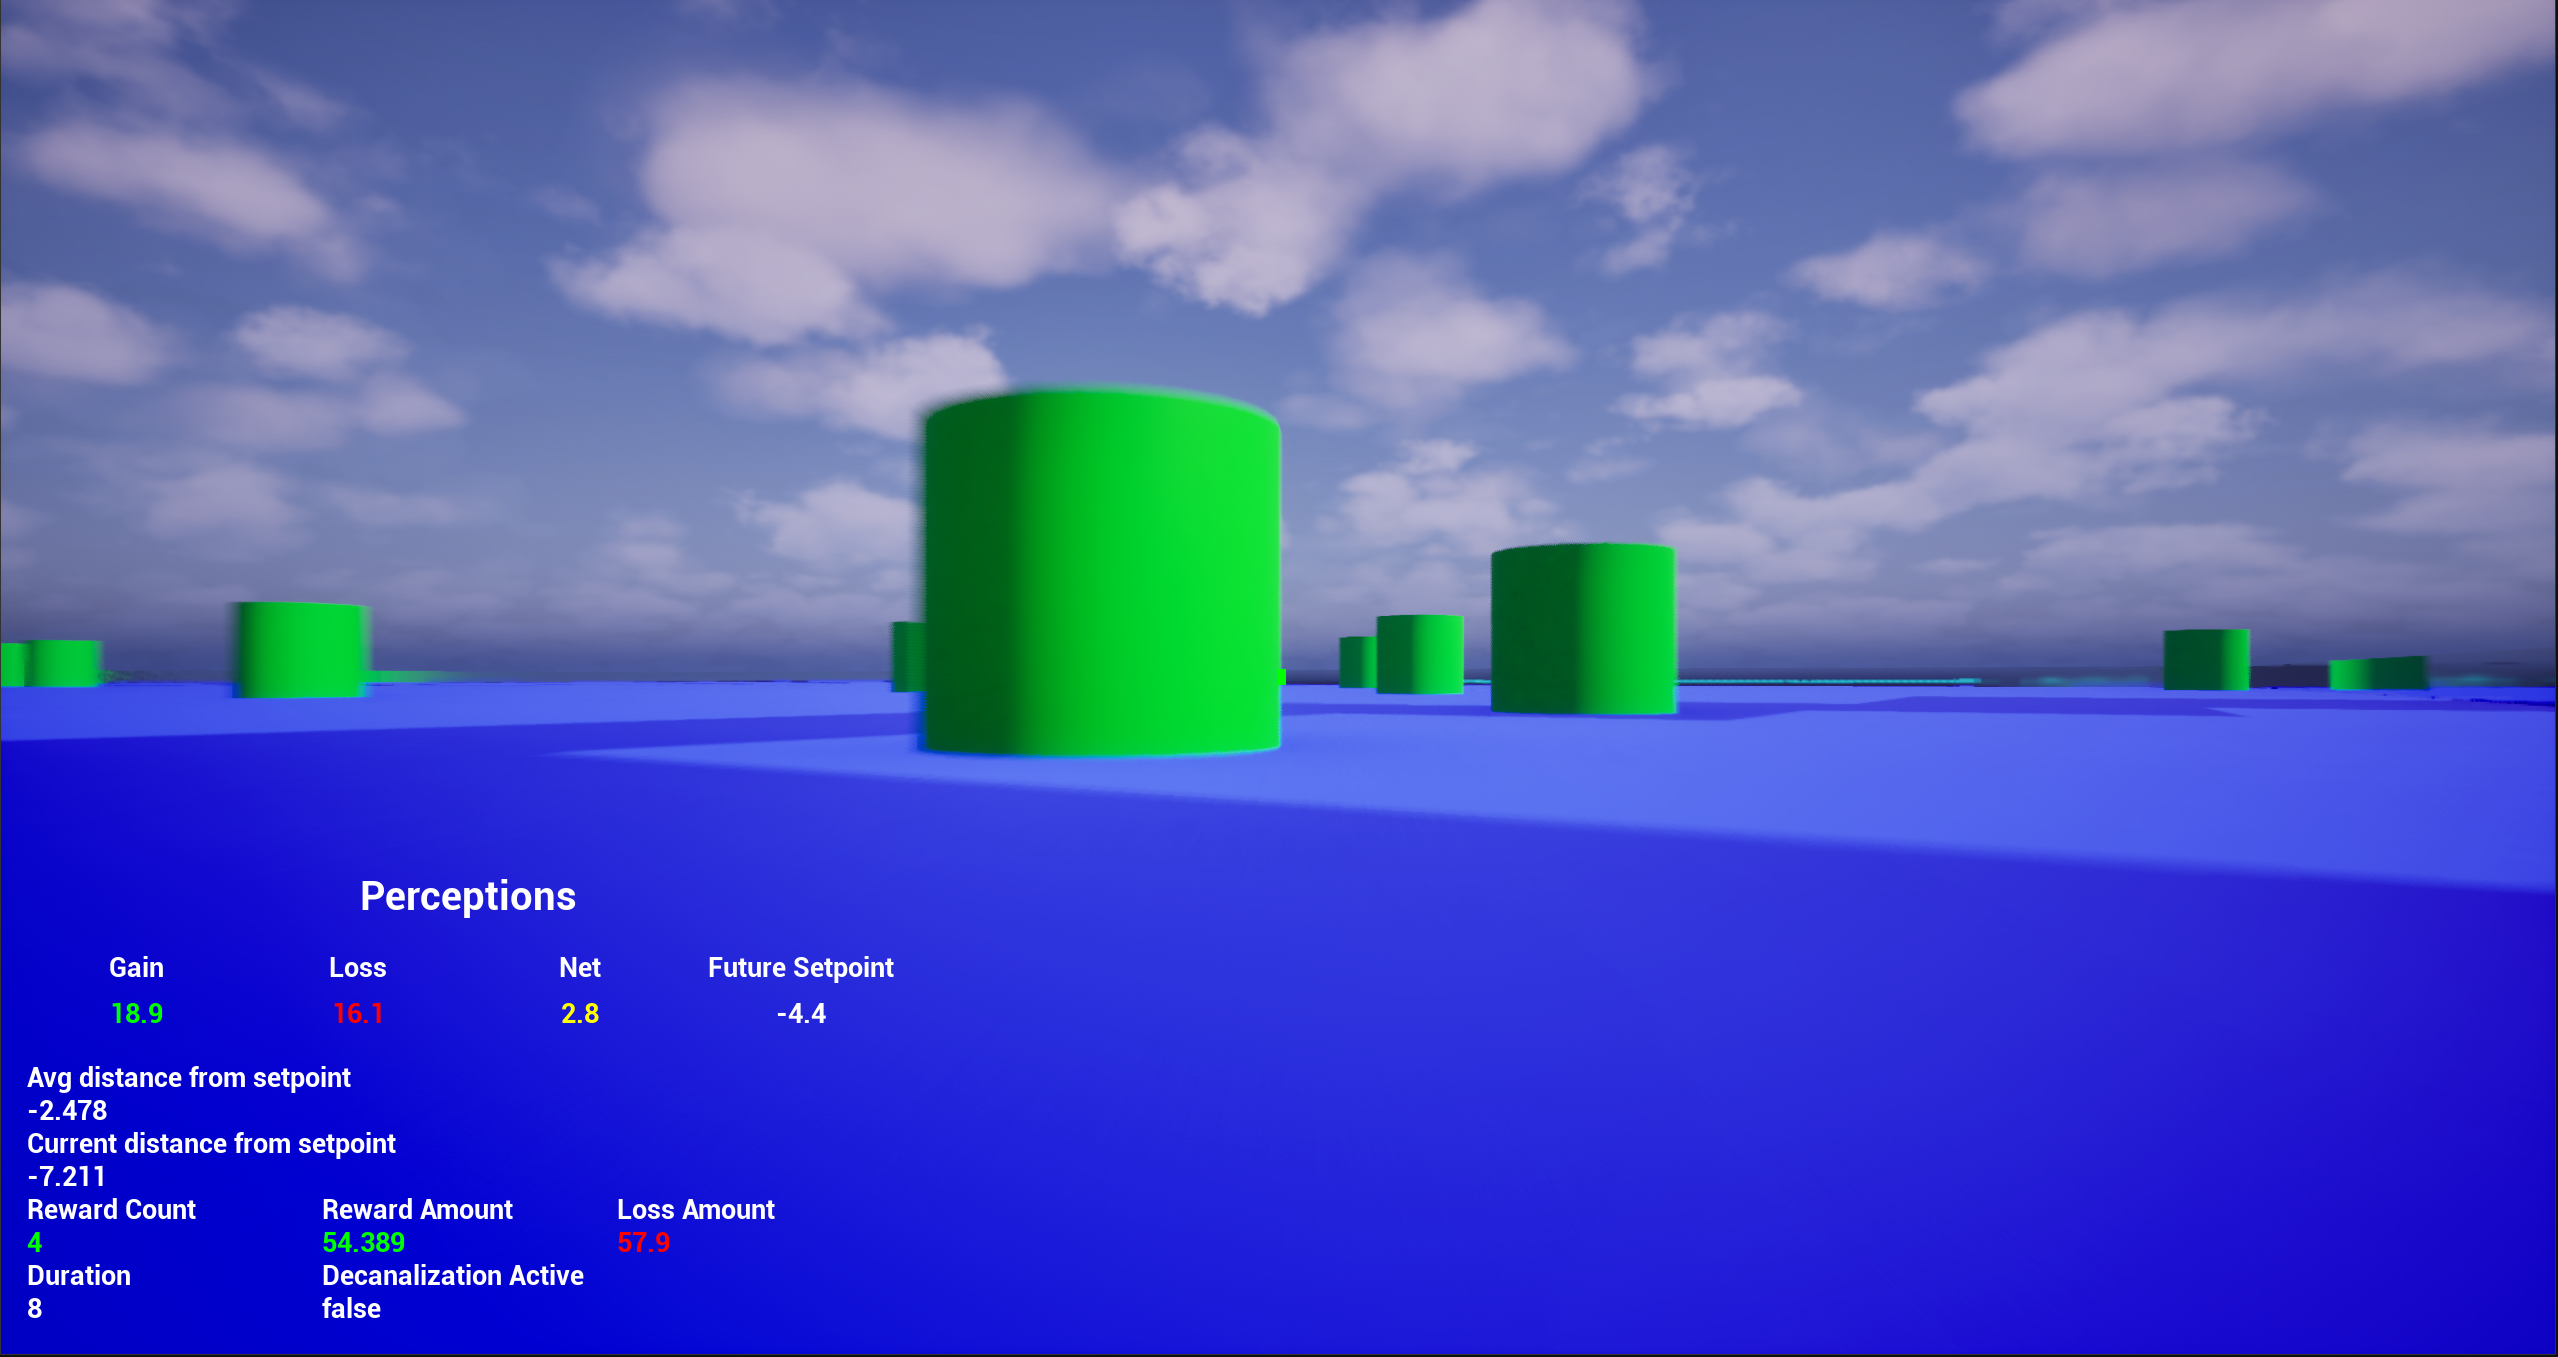
\includegraphics[width=1\linewidth]{figures/first-person.png}
    \caption{A first-person perspective from the agent's field of view (FOV). The agent can detect objects within this FOV and make predictions about the future value of \(h\), given the current value and the pellets and tiles that are in the current trajectory. The agent's perceptions are estimates. During decanalization, these estimates are altered such that all pellets are perceived as having equal homeostatic value. Likewise, all tiles are equally discounted (perceived as having a traversal cost of zero).}
\end{figure}

\subsection{Model Details}

The agent's state consisted of external (exteroceptive) and internal (interoceptive) values, including position, heading, velocity, and a limited, egocentric observation of the environment. Time $t$ corresponded to ticks or iterations of the simulations.

Externally, the agent perceived its current transform, its rotation in degrees and its x–y coordinates, as well as its instantaneous velocity in cm/s. It also detected nearby pellets and tiles via short-range raycasts, and registered whether its bounding box overlapped with any pellet. In addition, the agent computed a short-horizon prediction $\hat{h}$ of its future homeostatic value $h_{t+\kappa}$, based on its current heading, velocity, and the objects expected to lie along its projected path within a perception radius $\delta$.

Internally, the agent monitored a constant decremental drive $l$ applied to its homeostatic variable $h_t$ (this is a bit like hunger). It also tracked its current homeostatic state $h_t$, which was updated according to tile traversal costs, the baseline decremental $l$, and any increases caused by pellet consumption.

The agent was unaware of anything beyond these values and its actions taken (a floating point in \([-1,1]\), given each tick) over time, so its learning was contingent on finding useful interactions between the action (\(a\)) it takes at time \(t\) and the resulting future state at \(\mathbf{S}_{t+1}|a_t\)

Each iteration, an action was performed and a reward was calculated based on that action. The action space was limited to a single action, \(a\): rotate by one degree. This meant that a loop (total rotation input \(\pm 180^\circ\)) would, at minimum, have taken \(180\) ticks to execute.

The agent could perceive both a range of objects within an egocentric range of 180° of its current transform, as well as the potential homeostatic impact of objects directly in front of it, limited by the perception distance \(\delta\). At each time \(t\), we produced an array of seven raycasts from the agent's current transform. These were placed at -45, -30, -15, 0, 15, 30, and 45°, relative to the agent's current rotation, passing through all \(o\) and \(\tau\) objects, up to the perception distance range, \(\delta\). The agent used these observations to help make action decisions during and after training. Therefore, at any time \(t\), the agent was aware of:
\begin{itemize}
    \item All tiles \(\tau_t\) that intersected its raycasts
    \item All pellets \(o_t\) that intersected its raycasts
\end{itemize}

As with object perception and on top of passive loss over time, the agent also perceived both potential gain and loss to \(h\) through overlap with \(o\) and \(\tau\) objects, if it did not take any actions on its trajectory towards those objects from time \(t\) to the time it would reach them, given the agent's current velocity. To estimate this, we projected a single ray from the agent's current rotation to the perception distance range, \(\delta\). We call the potential \(h_{t+\kappa}\) value, \(\hat{h}\).

Let \(\mathbf{O} = \left\{ o_1,o_2,\ldots,o_{n} \right\}\) denote the pellet \(h\)-values intersected by the raycast at time \(t\), and let \(\mathbf{T} = \left\{\tau_1,\tau_2,\ldots,\tau_{m}\right\}\) denote the tiles intersected by the raycast at time \(t\). Then
\begin{equation}
    \begin{aligned}
        \hat{h}_t & = h_{t+\kappa}|(a_{[t, t+\kappa]}= \varnothing)                                                        \\
                  & = h_t + \sum_{o_i \in \mathbf{O}} o_{i} - \sum_{\tau_j \in \mathbf{T}} \hat{c}_{t}(\tau_j) - l(\kappa)
    \end{aligned}
\end{equation}
where
\begin{align*}
    o_{j}             & \quad\text{ is the }h \text{ value of a pellet}                               \\
    \hat{c}_{i}       & \quad\text{the predicted cost of moving through tile }i\text{ at time }t      \\
    \hat{h}_t         & \quad\text{ is the predicted value of } h\text{ at time } t                   \\
    a_{[t, t+\kappa]} & \quad\text{ are actions taken from time } t\text{ to } t+\kappa               \\
    \kappa            & \quad\text{ is the time it would take the agent to travel to the end }        \\
                      & \quad\text{of the raycast at the current velocity}                            \\
    l(\kappa)         & \quad\text{ is the sum of passive homeostatic loss over } \kappa \text{ time} \\
\end{align*}

Pellet instances (\(o_i\)) were represented as cylindrical objects that occupied the center of a tile and produced a positive effect on \(h\) on overlap with the agent. Each tile instance (\(\tau_i\)) produced a negative effect on \(h\) on overlap with the agent. The agent was represented as a cube with a bounding box that monitored and managed overlap with \(o\) and \(\tau\) objects.

Pellets were distributed randomly throughout the landscape at a fixed density (all sources of randomness were associated with a seed so that all simulation environments could be reproduced). Pellet locations were shuffled between training episodes and trial phases. The positive \(h\) value of each pellet (\(o_i\)) was set from a random value, within a range of 1 to 20. Throughout canalization phases, the value remained constant, and the agent could perceive this value when the pellet intersected with the agent's raycasts. During the decanalization phase, the value of each \(o_i\) became the set maximum possible \(\mathbf{O}\) value, \(20\). For training and running trials for analysis, we placed the agent in a deterministically random starting rotation and location, with an equal-density distribution of rewards. For training, we set the initial \(h\), \(h_0\), to \(-15\). In trials, \(-15 < h_0 < 15\). In training, this stochasticity helped prevent overfitting, where the agent would have devised a strategy that is not generally useful, resulting in brittle behavior that could easily be perturbed. In trials, this stochasticity presented different challenges to the agents, allowing us to observe their behavior more broadly.

The value \(h_{t+\kappa}\) of each tile \(\tau_i\) in the raycast (assuming the agent does not take an action and moves at a fixed linear velocity forward), was approximated in the implementation.

The agent was also taxed for traversing each tile, with the tax rate decreasing upon repeated traversals of that tile. This loosely aligns with the notion of ‘niche construction’, which suggests that organisms actively modify their environments to be better suited to their short and long-term needs \parencite{pio-lopez_scale-free_2025}. In doing so, organisms can effectively cultivate sources of homeostatic gain and loss \parencite{lyon_reframing_2021}. However, such behavior can also be interpreted as ecological canalization, which, alongside physiological canalization, leads to long-term exploitation that may or may not be optimal for overall flourishing, even though it might increase predictability and therefore decrease risk.

We represented different aspects of canalization in this simulation: canalization through learning to optimize internal setpoints with perception, and canalization through shaping the environment to improve predictability and reduce uncertainty. Agent training is itself a form of canalization, where the agent is shaped both by reinforcement and by the environment in which it learned. Although we do not presently explore actively updating agent behavior during or after decanalization, the training environment could be said to be partially constitutive of the agent, in the sense that the agent's canalization of the world alters the environment, such that it must use its formal learning to effectively learn novel behaviors in its new environment, without the agent having to alter itself internally. Of course, this form of environmental knowledge does not persist when the environment is altered.

To represent different degrees of canalization throughout the world, we created a grid of tiles that produced negative \(h\) (we call this movement tax ‘traversal cost’) each tick during which they overlapped with the agent. Each tile was tracked individually and started with the same initial traversal cost, which was discounted based on the number of times \(n\) the agent had overlapped with it. The traversal cost remained constant while the agent continued to overlap the same tile. The agent had to leave and return to the tile for that \(n\) to increase. Traversal cost was reduced at the rate of initial cost divided by the number of traversals.

Each tile was tracked individually. As the agent moved within the bounding box of an overlapping tile, the negative effect of the traversal cost was applied to \(h_{t+1}\). The agent also used this value to approximate future losses due to tile traversal. Total loss due to traversal was estimated after each action as the total loss from tiles that intersected with the agent's raycast, assuming \(n+1\) (i.e., that traversal would be discounted upon agent overlap). Performing a perfect prediction of future tile traversal-caused losses is computationally expensive, but we approximated this by gathering the future cost of each tile that collided with the raycast at time \(t\), then calculating the total number of movement timesteps (and therefore homeostatic loss) the agent would take to bisect these tiles through the hypotenuse (dividing the cost of the first and last tile that collide with the raycast by \(2\), as an average of the distance that remains to be covered), factoring in current velocity.

During decanalization, agent overlap \(n\) was incremented at a higher rate (3x the canalized rate). Post-decanalization, all tile overlap counts were reduced by a constant factor, resulting in \(n^{post} = \lfloor n^{pre} \cdot 0.5 \rfloor\) for each tile.

\subsection{Homeostatic Reinforcement Learning (HRL)}

Homeostatic Reinforcement Learning (HRL) models an agent that manages a set of internal physiological or cognitive variables (e.g., energy, temperature, hunger, curiosity). The agent's goal is to reduce drive $D$ by keeping these values close to a set of preferred setpoints \parencite{keramati_homeostatic_2014}:

\begin{equation}\label{eq:model-drive}
    D\left(H_t\right)=\sqrt[m]{\sum_{i=1}^N\left|h_i^*-h_{i, t}\right|^n}
\end{equation}
\(H^*=\left(h_1^*, h_2^*, ., h_N^*\right)\) is a vector of setpoints describing the organism's ideal physiological state and \(H_t=\left(h_{1, t}, h_{2, t} \ldots, h_{N, t}\right)\) represents the organism's actual physiological state at time \(t\). Note that for the case of $m = n = 1$, which is assumed here, $D$ is a sum of absolute values between the setpoints and the actual physiological states. We focus on the case of a single state \(h_t\), whose setpoint \(h^*\) is set to \(0\). This makes it easy to interpret $h$ values as either above or below the desired setpoint: if $h$ is food-satiation, then positive values are degrees of over-satiation and negative values are degrees of hunger. HRL rewards actions that increase or reduce $h$ over time in Goldilocks fashion, taking actions that make $h$ larger when it is below $h^*$ and taking actions that make $h$ smaller when it is above $h^*$.

Rewards were calculated based on the effect of the last action on \(h_t\). Most actions have a small impact on \(h_t\), being simply the sum of movement cost through the currently overlapping tile (\(\tau_i
\)) and constant decremental loss (\(l\)). When the agent consumes a pellet at time \(t\), however, \(h_{t} \gg h_{t-1}\).

We implemented the HRL reward function as
\begin{equation*}
    r^{HRL}_t =
    \begin{cases}
        \exp(-\alpha|h_t|),   & \text{if } |h_{t-1}| > |h_t| \\
        1 - \exp(\beta|h_t|), & \text{otherwise}             \\
    \end{cases} \\
\end{equation*}
where \(\alpha\) and \(\beta\) are scaling parameters. The agent was rewarded for decreasing \(|h|\) between timesteps, therefore approaching the \(h^*=0\) setpoint. The agent was punished for increasing its distance from the setpoint. The agent received disproportionately more reward the closer it got to a target. (This is a common practice when reinforcing behavior that approaches but never achieves the ideal state, which we address more in the discussion.)

Note that positive reinforcement for good behaviors is more effective in training than negative reinforcement, as focusing on the positive allows the agent to form new intentions, rather than merely warding it away from bad ones.

\subsection{Homeostatic Negative Feedback (NF)}

We also trained and measured the performance of agents that used a negative feedback (NF) reward function, which only takes actions when \(h_t\) is \emph{less} than the ideal setpoint \(h^*_t\). A heater thermostat provides a classic example: if the thermostat is set to $68^\circ\ \mathrm{F}$, the heater will only come on when the temperature falls below that. No actions are taken when the temperature is above \(h^*_t\).

We chose NF as a contrast to HRL because, unlike HRL, agents that rely on NF are incapable of taking anticipatory actions. Without being able to anticipate changes to their environments as a consequence of their actions, NF agents should see significantly greater deviation from the ideal setpoint, \(h^*_t\). Decanalization might therefore have little to no effect on performance, as the NF-trained agent should not fully benefit from the long-term prediction benefits that we should anticipate for HRL-trained agents.

To model NF as a reward function, we rewarded actions that increased \(h_t\) and punished actions that decreased \(h_t\) when \(h_t < 0\). In contrast to HRL, when \(h_t > 0\), we provided neither punishment nor reward for actions.

\begin{equation*}
    r^{NF}_t =
    \begin{cases}
        0,                       & \text{if } h_{t-1} >= 0 \text{ and } h_t >= 0                                   \\
        \beta \cdot h_t,         & \text{if } h_{t-1} >= 0 \text{ and } h_t < 0                                    \\
        \alpha|h_{t-1}|,         & \text{if } h_{t-1} < 0 \text{ and } h_t >= 0                                    \\
        \alpha(|h_t|-|h_{t-1}|), & \text{if } h_{t-1} < 0 \text{ and } h_t < 0 \text{ and } |h_{t-1}| - |h_t| >= 0 \\
        \beta(|h_t|-|h_{t-1}|),  & \text{if } h_{t-1} < 0 \text{ and } h_t < 0 \text{ and } |h_{t-1}| - |h_t| < 0
    \end{cases} \\
\end{equation*}
where \(\alpha\) and \(\beta\) are scaling values. The first case captures the difference from HRL: no rewards are given above the setpoint. The second case applies a penalty for falling below the setpoint that is proportional to how far below the agent falls. The third case rewards recovery. The fourth case rewards getting closer to the setpoint when below it. The final case penalizes moving farther from the setpoint when below it.

\subsection{Learning via Proximal Policy Optimization (PPO)}

As noted above, agents were trained using model-free reinforcement learning to optimize their respective reward functions (HRL or NF). We used a standard implementation of PPO (\cite{schulman_proximal_2017}) associated with the Pytorch backend of Unreal Engine’s Learning Agents interface.

Training episodes continued until 60 seconds elapsed or \(|h_t| > 50\), at which point the agent was reset and a new training episode began.  Once 60 seconds elapsed, the episode was terminated at time \(t\) and future rewards were estimated by bootstrapping from the value function, $\hat{r}_t = r_t + \gamma V(s_{t+1})$, where \(\hat{r}\) was the best estimate of the future reward that would have been given if the agent had been allowed to continue, and where $\gamma \in [0, 1]$ is a discount factor. At the end of each episode, tile traversal counts were reset and the agent's position was randomized. \(h_0\) was also reset to its initial value of \(-15\).\footnote{The value of  \(-15\) was chosen because the HRL reward function was found to benefit from early punishment during training. With a negative starting value, each agent was immediately pressured to find pellets, making shorter training cycles possible and thus improving the learning rate. This is just a practical implementation consideration for training efficiency, however—HRL lets agents learn with different starting \(h_0\) values, although extreme positive or negative initial values greatly limit practical learning performance.}

\subsection{Canalization and Decanalization}

During trials, the agent first canalized the tiles, carving out low-cost pathways as it maximized the rewards received. After the canalization phase, we simulated decanalization by altering the perception of objects in the tiles that affected \(h\), as well as the rate and depth of canalization. After this decanalized movement phase, we returned agent perception to its initial parameters.

We modeled decanalization by temporarily altering several parameters of the environment, as well as the agent’s perception. During the decanalization phase, pellets (\(o_i\)) were set to being perceived as having the maximum possible positive effect on \(h\), flattening differences in their reward value. Tiles (\(\tau_i\)) were set to being perceived as having zero traversal cost, encouraging unconstrained exploration. The rate of canalization was also increased threefold, so that each tile’s visitation count accumulated more quickly, reflecting heightened metaplasticity. Finally, when the decanalization period ended, all tile traversal counts were halved to represent reduced depth of canalization across the landscape. These decisions were motivated by the characterization of decanalization by \citeauthor{juliani_deep_2024} (\citeyear{juliani_deep_2024}).

This table shows how the phases were organized:
{\scriptsize
\[
    \begin{array}{|c||c|c|c|}
        \hline
         & \text{Phase 1}        & \text{Phase 2}   & \text{Phase 3}    \\
         & t\in[0,6000]          & t\in(6000,12000] & t\in(12000,18000] \\
        \hline
        \text{Decanalization condition (CDR)}
         & \text{Canalization}
         & \text{Decanalization}
         & \text{Recanalization}                                        \\
        \hline
        \text{No-decanalization condition (CCC)}
         & \text{Canalization}
         & \text{Canalization}
         & \text{Canalization}                                          \\
        \hline
    \end{array}
\]
}

For each reward function (HRL and NF), we trained multiple agents from independent random seeds. Across seeds, agents converged on qualitatively similar policies and showed similar end-of-training performance. We therefore focus in the main text on aggregate trial-level performance under each condition, using individual trained agents primarily for visualization and qualitative illustration.

Between phases, we reset the agent's homeostatic state \(h\) to a random value in \([-15,15]\). This prevented phase comparisons from being driven by carryover in the agent's immediate internal state and allowed us to evaluate behavior from a range of initial conditions. The aim was to test whether canalization and decanalization altered subsequent behavior across matched environments, rather than to model persistent within-trial carryover in \(h\).

Across matched comparisons between the decanalization (CDR) and no-decanalization (CCC) conditions, agents were evaluated on identical environment instances. Within each paired comparison, the same seeded pellet arrangement and starting transform were used in both conditions, with the phase-specific decanalization manipulation as the only intended difference. Across trials, these seeds varied, so each trial presented a different environment instance drawn from the same generation procedure.

These choices were inspired by \citeauthor{juliani_deep_2024} (\citeyear{juliani_deep_2024}), which cleanly separates canalization into inference and learning, with decanalization being a state of increased meta-plasticity for both. In this paradigm, the behavioral landscape is flattened, resulting in a similar flattening of reward (all sources of reward are perceived as roughly equivalent), a discounting of cost (the flattened landscape affords frictionless movement), an increase in learning rate (the locations traversed during decanalization carve out a deeper path than usual), and a decrease in canalization depth (the entire landscape is partially “forgotten”, as all previously traversed paths are smoothed out). Decanalization is explained in more detail in the discussion.

\subsection{Statistical Analysis and Reproducibility}

For each reward function, we trained multiple agents from independent random seeds and observed similar converged behavior across seeds. Evaluation then consisted of matched comparisons between decanalization (CDR) and no-decanalization (CCC) conditions, using identical seeded environment instances within each pair. Reported summary measures were captured at the end of each phase. We report mean differences, $p$-values, and Cohen's $d$ as compact summaries of these paired condition comparisons.

Because several outcome measures are related and the present study is intended primarily as a proof-of-principle computational analysis, the inferential statistics should be interpreted as descriptive support for broader behavioral patterns rather than as the sole basis for the paper's claims. Accordingly, we emphasize consistency across matched trials, effect sizes, and convergence across independently trained seeds. All stochastic elements of training and evaluation were seed-controlled so that environment generation, initial transforms, and condition matching could be reproduced from the recorded parameter settings.

\section{Results}\label{model-results}

We compared two different versions of the trained agents (HRL and NF) under two conditions: decanalization and no-decanalization. The four experimental conditions were therefore: HRL with decanalization, HRL  without decanalization, NF with decanalization, and NF without decanalization. Unless otherwise noted, condition comparisons were conducted on matched environment seeds so that differences between CDR and CCC reflect the decanalization manipulation rather than differences in pellet layout or starting position.

\begin{figure}
    \centering
    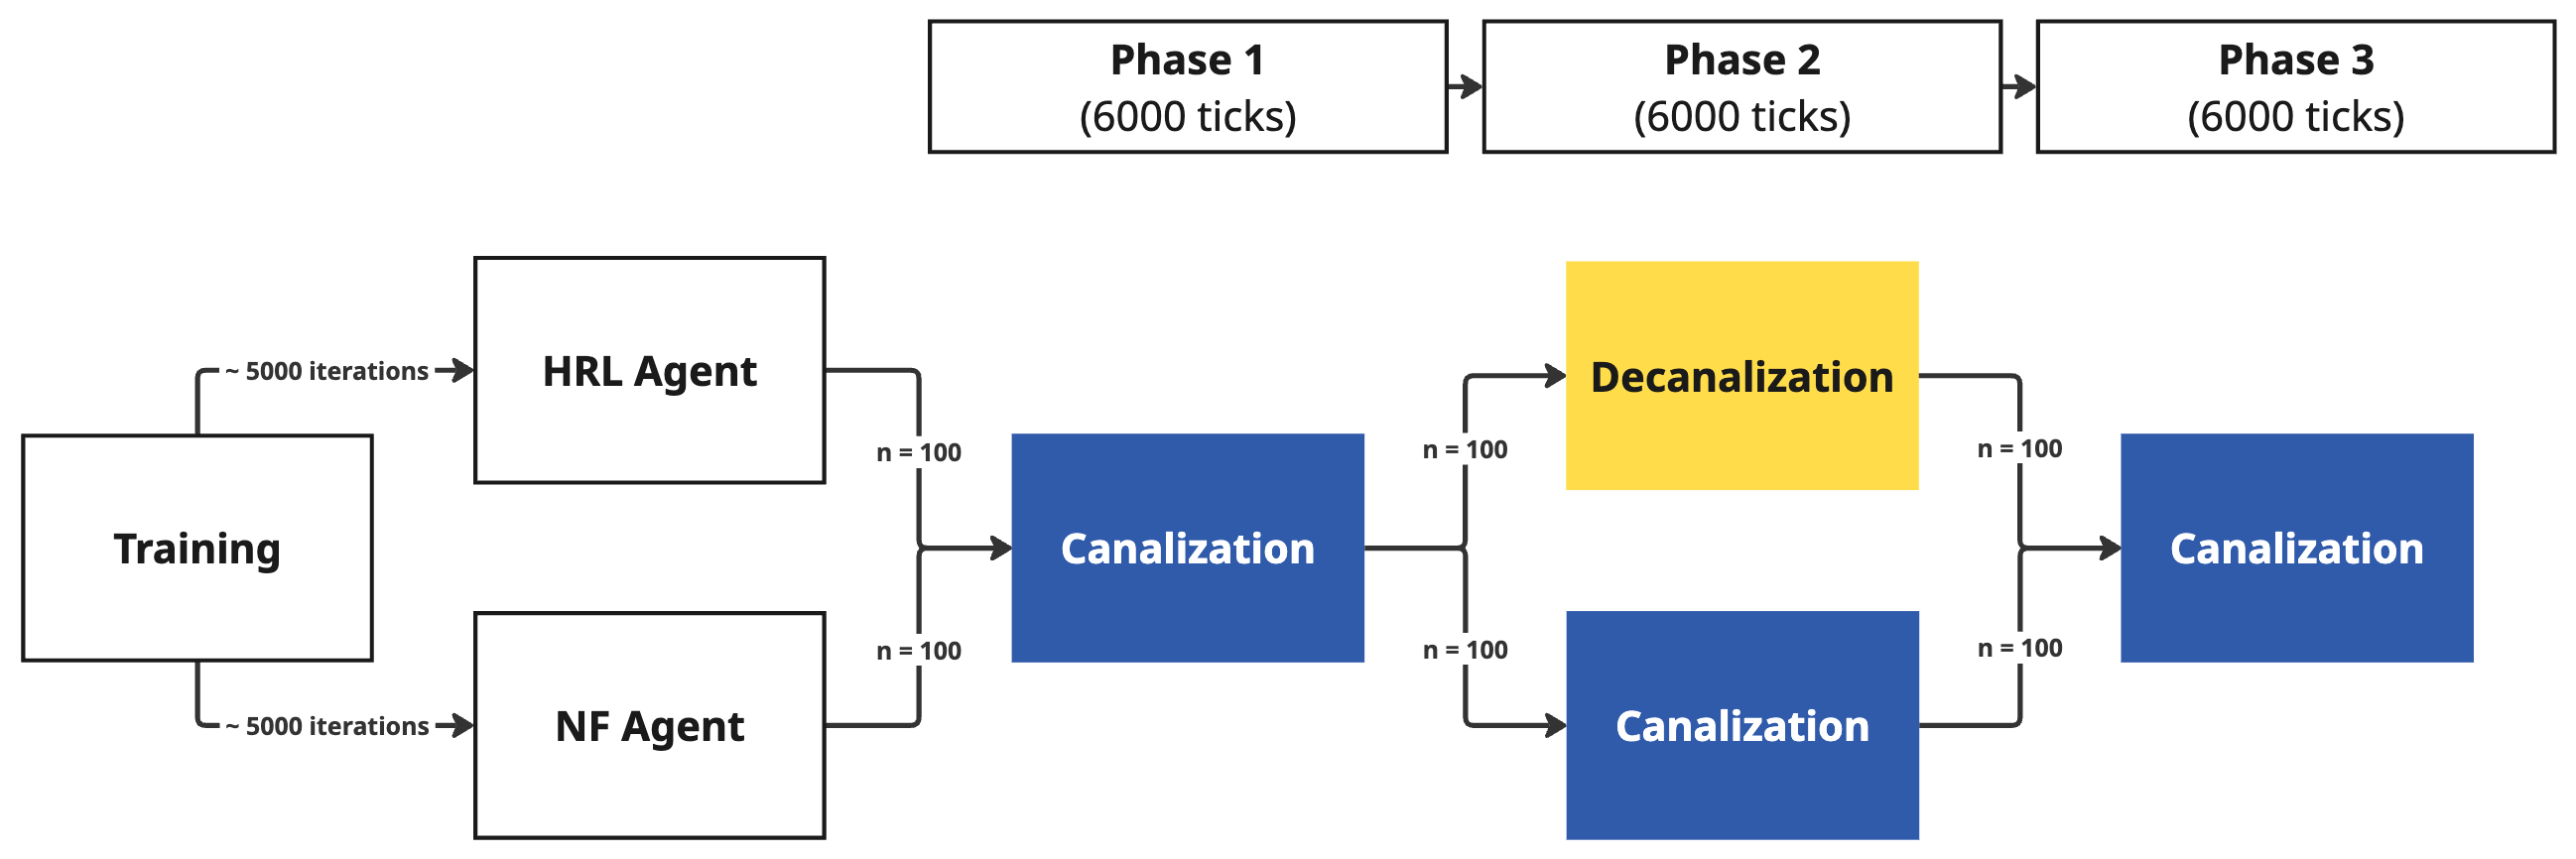
\includegraphics[width=0.75\linewidth]{figures/modeling-process.png}
    \caption{Simulation setup: Across matched CDR and CCC comparisons, agents were evaluated on identical environment instances. The same seeded pellet arrangement and starting transform were used in both conditions, with the phase-2 decanalization manipulation as the only difference. Across trials, these seeds varied, so each trial presented a different environment instance drawn from the same generation procedure.}
\end{figure}

Recall that each agent was trained with reinforcement learning to maximize the rewards it received, which were awarded proportionately to the distance of the agent from \(h_*\), where \(h_* = 0\). Strongly positive or negative means and large deviations in either direction would suggest that the agent is not performing actions that maximize its rewards.

\subsection{HRL: decanalization vs. control}

\begin{table}
    \centering
    \scriptsize
    \setlength{\tabcolsep}{2.5pt}
    \resizebox{\linewidth}{!}{
        \begin{tabular}{|l|
                >{\columncolor[HTML]{E4EEFC}}l|
                >{\columncolor[HTML]{E4EEFC}}l|
                >{\columncolor[HTML]{E4EEFC}}l|
                >{\columncolor[HTML]{FFE6E5}}l|
                >{\columncolor[HTML]{FFE6E5}}l|
                >{\columncolor[HTML]{FFE6E5}}l|
                >{\columncolor[HTML]{E4EEFC}}l|
                >{\columncolor[HTML]{E4EEFC}}l|
                >{\columncolor[HTML]{E4EEFC}}l|}
            \hline
            \textbf{Phase Comparison} & \multicolumn{3}{|l|}{\cellcolor[HTML]{E4EEFC}\textbf{CDR-1 vs CCC-1}} & \multicolumn{3}{|l|}{\cellcolor[HTML]{FFE6E5}\textbf{CDR-2 vs CCC-2}} & \multicolumn{3}{|l|}{\cellcolor[HTML]{E4EEFC}\textbf{CDR-3 vs CCC-3}}                                                                                                         \\ \hline
            \textbf{Measure}          & \textbf{\(\Delta\)M}                                                  & \textbf{p}                                                            & \textbf{d}                                                            & \textbf{\(\Delta\)M} & \textbf{p} & \textbf{d} & \textbf{\(\Delta\)M} & \textbf{p-value} & \textbf{d} \\ \hline
            \(h\) mean                & -16.96                                                                & 0.0324*                                                               & -0.4342                                                               & 262.57               & 0.0000***  & 6.2267     & -42.77               & 0.0000***        & -1.0640    \\ \hline
            \(h\) deviation           & -742.02                                                               & 0.0529                                                                & -0.3918                                                               & 12927.72             & 0.0000***  & 6.2509     & -1847.65             & 0.0000***        & -0.9336    \\ \hline
            Reward pred.              & 0.2121                                                                & 0.9623                                                                & 0.0095                                                                & -0.0728              & 0.0000***  & -5.3206    & 0.2400               & 0.0114*          & 0.5160     \\ \hline
            \(h\) lost                & -6.97                                                                 & 0.3262                                                                & 0.1973                                                                & 122.64               & ---        & ---        & 39.77                & 0.0001***        & 0.8255     \\ \hline
            \(h\) gained              & -34.43                                                                & 0.0186*                                                               & -0.4788                                                               & 159.35               & 0.0000***  & 2.0970     & -45.75               & 0.0020**         & -0.6341    \\ \hline
            Unique pellets            & -1.30                                                                 & 0.3868                                                                & -0.1739                                                               & 10.52                & 0.0000***  & 1.3959     & 0.84                 & 0.6223           & 0.0988     \\ \hline
        \end{tabular}}
    \caption{T-tests for comparisons between dependent measures for HRL in decanalization (CDR) and no-decanalization (CCC) conditions. Values were captured at the end of each phase, just before switching the rest. ‘\(\Delta\)M’ is the change in mean value (the value of CDR minus the value of CCC). ‘d’ refers to Cohen's d. ‘*’ indicates $p < .05$, ‘**’ indicates $p < .01$, and ‘***’ indicates $p < .001$. Measures are discussed in the main text.  The $p$ and $d$-values for \(h\) lost in phase 2 are excluded, as having no perception of \(h\) loss was part of decanalization.}
    \label{model-analysis-hrl}
\end{table}

Table \ref{model-analysis-hrl} shows a comparison of 6 measures, where the CDR condition is compared with the CCC condition. In effect, these are comparisons of the form “treatment condition – control condition”, so negative values indicate that more of something occurred in the control condition. A negative $h$-mean indicates that the agent was more “hungry” in the control condition. A negative $h$-deviation indicates that there was more variance in hunger in the control condition. ‘Reward pred.’ is short for the total normalized reward prediction (what an agent would be rewarded for its actions if it were being trained). Positive ‘Reward pred’ indicates that the agent in the control condition predicted that it would receive a smaller reward. Negative $h$-lost indicates that more new paths were taken in the control condition (passive loss is the same in each case, so this measure tracks traversal costs). ‘\(h\) gained’ is the average total \(h\) increase from pellets, while ‘Unique pellets’ is the average number of different pellets (i.e., pellet diversity) consumed by the agent during the phase. Negative $h$ gained signifies that the agent received fewer/lower-value pellets in the control condition. Negative unique pellets indicates that the agent received more unique pellets in the control condition; positive unique pellets signifies that the agent received more unique pellets in the treatment condition.

Performance differences in phase 1 were minimal, as expected, as the phases were identical. There was a small but significant difference in mean \(h\) and total \(h\) gained. Although agents started in the same world with the same tile arrangement, their learned behavior has randomness built in, and the result was a type 1 error; a false positive. The other measures did not change significantly, as expected.

During phase 2 (decanalization vs. canalization), we observed significant differences in all measures. This was expected, given the changes in perception of pellet value, tile traversal cost, and canalization rate. The decanalized agent collected pellets more greedily (159.35 more \(h\) gain on average) and with a higher diversity of pellets (10.52 more unique pellets harvested on average).

The phase 3 (recanalization vs. canalization) comparison was critical, as it directly compared agents that underwent or did not undergo a decanalization phase. The agent in the recanalization condition performed significantly better at managing its mean \(h\), relative to \(h^*\), as well as lowering its setpoint deviation (measured as the standard deviation over all timesteps in the phase), relative to the no-canalization agent. The predicted reward performance of the decanalized agent slightly increased, although it experienced more loss in \(h\), post-decanalization. This increased loss was offset by greater \(h\) increase (through pellet consumption), although the diversity of pellets consumed did not increase, suggesting that decanalized agents spontaneously located higher-payout pellets in less-traversed regions.

These results suggest that decanalization can lead to spontaneous exploration of new pathways, resulting in improved homeostatic performance. The decanalized agent modestly improved its reward performance, which was reflected in its improved ability to stay close to the setpoint.

\subsection{NF: decanalization vs. control}

The effects of decanalization on the NF-trained agent were much less pronounced.
\begin{table}
    \centering
    \scriptsize
    \setlength{\tabcolsep}{2.5pt}
    \resizebox{\linewidth}{!}{
        \begin{tabular}{|l|
                >{\columncolor[HTML]{E4EEFC}}l|
                >{\columncolor[HTML]{E4EEFC}}l|
                >{\columncolor[HTML]{E4EEFC}}l|
                >{\columncolor[HTML]{FFE6E5}}l|
                >{\columncolor[HTML]{FFE6E5}}l|
                >{\columncolor[HTML]{FFE6E5}}l|
                >{\columncolor[HTML]{E4EEFC}}l|
                >{\columncolor[HTML]{E4EEFC}}l|
                >{\columncolor[HTML]{E4EEFC}}l|}
            \hline
            \textbf{Phase comparison} & \multicolumn{3}{|l|}{\cellcolor[HTML]{E4EEFC}\textbf{CDR-1 vs CCC-1}} & \multicolumn{3}{|l|}{\cellcolor[HTML]{FFE6E5}\textbf{CDR-2 vs CCC-2}} & \multicolumn{3}{|l|}{\cellcolor[HTML]{E4EEFC}\textbf{CDR-3 vs CCC-3}}                                                                                                   \\ \hline
            \textbf{Measure}          & \textbf{\(\Delta\)M}                                                  & \textbf{p}                                                            & \textbf{d}                                                            & \textbf{\(\Delta\)M} & \textbf{p} & \textbf{d} & \textbf{\(\Delta\)M} & \textbf{p} & \textbf{d} \\ \hline
            \(h\) mean                & -6.475                                                                & 0.2770                                                                & -0.2186                                                               & 255.35               & 0.0000***  & -4.7056    & -17.20               & 0.0794     & -0.3545    \\ \hline
            \(h\) deviation           & -92.90                                                                & 0.6706                                                                & -0.0853                                                               & 11629.61             & 0.0000***  & 5.0702     & -595.34              & 0.1552     & -0.2865    \\ \hline
            Reward pred.              & -0.1404                                                               & 0.0000***                                                             & -1.0695                                                               & 0.131                & 0.0063**   & 0.5587     & -0.1702              & 0.0000***  & -1.1767    \\ \hline
            \(h\) lost                & 3.302                                                                 & 0.3779                                                                & 0.1772                                                                & 163.4                & ---        & ---        & 31.600               & 0.0003***  & 0.7499     \\ \hline
            \(h\) gained              & -12.93                                                                & 0.2211                                                                & -0.2463                                                               & 100.65               & 0.0000***  & 1.2309     & -2.636               & 0.8457     & -0.0390    \\ \hline
            Unique pellets            & 1.020                                                                 & 0.3370                                                                & 0.1930                                                                & 1.500                & 0.2260     & 0.2437     & 1.680                & 0.2666     & 0.2234     \\ \hline
        \end{tabular}}
    \caption{T-tests for comparisons between dependent measures for NF in decanalization (CDR) and no-decanalization (CCC) conditions. Note that there are less significant comparisons in the last column than in the HRL case.}
    \label{model-analysis-nf}
\end{table}

As with HRL and as expected, phase 1 performance was flat—even flatter with NF, possibly due to the simplicity of its reward function. We again saw a false positive here, this time in terms of predicted reward.

Phase 2 performance was similar to HRL's performance, with the decanalized agent exhibiting increased deviation from the setpoint as it greedily pursued pellets, although it did not increase the diversity of pellets it pursued—it instead tended to exploit the same pellets. We saw a modest effect on reward prediction here. Given the opposite effect in the first phase, this suggests that predicted reward might have been sensitive to the inherent randomness in agent actions and/or poor reward prediction.

Phase 3 performance of the decanalization versus no-decanalization agent in phase 3 was strikingly different from what we saw with HRL. \(h\) mean performance difference was marginally significant, with the decanalized agent staying a bit closer to 0, suggesting improved performance. Most of the other results were flat across conditions, with the strong exceptions of predicted reward and \(h\) lost, where the decanalized agent saw a significantly lower predicted reward and a higher loss in \(h\). As with HRL, this could suggest that decanalization can result in pushing the agent into a less-explored region of the landscape. However, unlike HRL, RL-trained agents do not appear to benefit in the homeostatic sense discussed here. They were pushed outside their trajectories, but they did not spontaneously identify pathways that could improve their homeostatic performance—in their case, taking actions to keep their \(h\) value above zero.

\subsection{HRL vs. NF after decanalization}
\begin{table}
    \centering
    \scriptsize
    \setlength{\tabcolsep}{2.5pt}
    \resizebox{\linewidth}{!}{
        \begin{tabular}{|l|
                >{\columncolor[HTML]{E4EEFC}}l|
                >{\columncolor[HTML]{FFE6E5}}l|
                >{\columncolor[HTML]{E4EEFC}}l|}
            \hline
            \textbf{Phase comparison}
                            & \multicolumn{1}{|l|}{\cellcolor[HTML]{E4EEFC}\textbf{\(\Delta\)HRL-1 vs \(\Delta\)NF-1}}
                            & \multicolumn{1}{|l|}{\cellcolor[HTML]{FFE6E5}\textbf{\(\Delta\)HRL-2 vs \(\Delta\)NF-2}}
                            & \multicolumn{1}{|l|}{\cellcolor[HTML]{E4EEFC}\textbf{\(\Delta\)HRL-3 vs \(\Delta\)NF-3}}                                                                  \\ \hline

            \textbf{Measure}
                            & \textbf{\(\Delta\)M}
                            & \textbf{\(\Delta\)M}
                            & \textbf{\(\Delta\)M}                                                                                                                                      \\ \hline

            \(h\) mean      & \multicolumn{1}{|l|}{-10.49}                                                             & \multicolumn{1}{|l|}{7.22}    & \multicolumn{1}{|l|}{-25.57}   \\ \hline
            \(h\) deviation & \multicolumn{1}{|l|}{-649.12}                                                            & \multicolumn{1}{|l|}{1298.11} & \multicolumn{1}{|l|}{-1252.21} \\ \hline
            Reward pred.    & \multicolumn{1}{|l|}{0.353}                                                              & \multicolumn{1}{|l|}{-0.204}  & \multicolumn{1}{|l|}{0.41}     \\ \hline
            \(h\) lost      & \multicolumn{1}{|l|}{3.668}                                                              & \multicolumn{1}{|l|}{-40.76}  & \multicolumn{1}{|l|}{8.17}     \\ \hline
            \(h\) gained    & \multicolumn{1}{|l|}{-21.50}                                                             & \multicolumn{1}{|l|}{58.70}   & \multicolumn{1}{|l|}{-43.11}   \\ \hline
            Unique pellets  & \multicolumn{1}{|l|}{2.32}                                                               & \multicolumn{1}{|l|}{9.02}    & \multicolumn{1}{|l|}{-0.84}    \\ \hline
        \end{tabular}}
    \caption{The effects of decanalization on HRL vs NF-trained agents, captured as the difference of differences between HRL and NF-trained agents across the three phases (e.g., the mean \(h\) difference for HRL with and without decanalization, subtracted by the mean \(h\) difference for NF with and without decanalization).}
    \label{model-analysis-hrl-vs-nf}
\end{table}
Despite the shared series of trial configurations, only HRL-trained agents saw homeostatic performance benefits from decanalization.

If we compare the effects of decanalization on both agents, we observe that HRL-trained agents saw greater \(h\) mean deviation in all three phases, but were better able to remain close to the ideal homeostatic setpoint, \(h_*\). During decanalization, we clearly see the greedy, exploratory preference of the HRL-trained agent, which pursued and consumed a greater diversity of pellets.

Focusing on the post-decanalization results, only HRL agents were able to improve their reward performance. HRL-trained agents did this with fewer unique pellets and a lower per-pellet gain, suggesting that they zeroed in on pellets that could reduce their deviation from the setpoint, which was greatly reduced from the baseline. This was accompanied by a higher \(h\) loss rate, demonstrating that the HRL-trained agents pursued low-payout pellets in less-exploited regions. In contrast, NF-trained agents actually saw a decrease in reward after decanalization, greedily and erratically consuming pellets. In summary, decanalization greatly improved the homeostatic performance of HRL-trained agents and did not improve the performance of NF-trained agents—instead, it made them worse.

\subsection{Summary}

We observed that decanalization had a strong impact on agent behavior, particularly the HRL-trained agent, which improved its performance without the need for internal relearning through weight adjustment. Instead, temporary changes to its perception of the environment were sufficient to nudge the agent towards regions and rewards that reduced the average distance and deviation from the setpoint. Performance with the NF-trained agent was more mixed. Although the NF agent was able to competently stay above the setpoint during recanalization, it actually saw increased \(h\) variation. Moreover, it greedily consumed pellets, to the extent that its rewards decreased, as its \(h_t\) was well above \(h_*\) as a consequence of this (i.e., it could not be rewarded because it was too far above the setpoint). For NF, decanalization increased exploitation. Decanalization had a markedly different effect on the HRL-trained agent. Post-decanalization, the agent improved its performance. It reduced its pellet consumption, increased both its homeostatic loss and gain, kept itself closer to the  ideal \(h_*\), and decreased the variation of \(h\).

\section{Discussion}\label{model-discussion}

Using HRL and NF as comparative reward functions and PPO for optimization, we simulated a canalization, decanalization, and recanalization process. Agents were trained to minimize the distance from the setpoint (HRL) or to return to the setpoint once they detected that they were below it (NF). To further entrench agents and simulate learning under stress and uncertainty, which is often what precipitates hypercanalized pathologies such as depression, we made repeated traversal less costly. The interaction of discounted repeated movement, passive costs, and homeostatic rewards canalized agent behaviors. Although these behaviors were locally effective at maximizing rewards and minimizing punishments, they were far from the ideal behaviors available in the world, both in terms of reward maximization and in terms of the stated ideal of setpoint-distance minimization. By introducing a temporary state of decanalization, agents spontaneously escaped hypercanalized areas of the world, entering an exploratory space and forming new paths. This decanalized state was not well-suited to setpoint-distance minimization but led to improved performance after the initial set of parameters were restored. With this simulation, we helped demonstrate that this slow degradation of homeostatic performance over time could be mitigated by introducing decanalization.

Decanalization assisted agents in pursuing their homeostatic goals. By altering their perception and canalization rate, agents were spontaneously shifted from exploitative to exploratory behavior, without requiring explicit relearning. This resulted in improved performance, measured as distance from a homeostatic setpoint.

The introduction of a decanalization phase improved HRL-trained agent performance but did not directly improve NF-trained agent performance. Neither agent performed optimally in terms of high-level strategy, although HRL-trained agents came close. Given our design, the optimal strategy to minimize \(h\) mean and setpoint deviation would have been to identify one or a few minimal-payout pellets (through exploration) and to repeatedly harvest those by looping around those regions in an exploitative fashion. The HRL-trained agent did part of this well, as it correctly identified that low-payout pellets would result in decreased \(h\) variance. It did not fully optimize its behavior, however, as \(h\) mean and variance were not close to the theoretical ideal of zero. Still, they were significantly closer to zero than both the control condition and to both varieties of NF-trained agents.

NF-trained agents did not see significant performance improvements with decanalization. With NF, the agent is rewarded only when \(h < 0\) and it consumes a pellet, so the only risk of over-consumption is an imperceptible loss of possible reward. This differs from HRL, where taking actions to increase the distance from \(h_*\) is directly punished. NF is easier to satisfy and does not directly punish poor performance. Although decanalization was implemented in the same way as it was for HRL, the immediate effect of decanalization on NF-trained agents was extreme exploitation, where agents indiscriminately and greedily sought out and exploited proximate rewards. In contrast, HRL-trained agents went from being locally canalized to openly exploring the wider world throughout decanalization. When we removed the effects of decanalization, they benefited from the world knowledge and pathways they gained through exploration, finding more-ideal pellets to exploit.

\subsection{Criticality and metastability in HRL}

Decanalization has ties to criticality. \cite{lepow_critical_2021} (\citeyear{lepow_critical_2021}) posits that psychedelics can precipitate critical period plasticity similar to plasticity in early development, leading to “exquisite sensitivity to environmental input.” This mirrors \cite{juliani_deep_2024}'s description of acute shifts to inference, which, when supported by heightened metaplasticity, result in learning and relearning of the environment and actions that can manipulate it—made even stronger when the environment itself shifts during these critical periods.

To minimize setpoint deviation over time, the agent's ideal solution should have been to explore the space until it found the pellet with the lowest \(h\), then canalize and exploit that pellet with cyclical loops through tiles that perfectly offset the net positive effect of the pellet on \(h_t\). Such an agent would have effectively minimized setpoint distance and received exponentially greater rewards as a result. However, in real-world environments, endlessly exploitable resources, perfect predictions, and environmental constancy are improbable. Moreover, the optimal reward is often unknown, and setpoints—as in allostasis \parencite{sterling_allostasis_1988}—are themselves changing over time. Organisms have to deal with many trade-offs and risks—learning to use drive to motivate discounted behaviors that are well-adapted to long-term survival means being able to live with non-ideal states.

\subsection{Limitations}

One limitation of this model is that it only explores the management of a single setpoint. Living organisms coordinate around the management of many different setpoints, presenting constant pressure for organisms to effectively juggle these, allowing some to stray far from the ideal range so that others may be satisfied. In such cases, the far-from-ideal setpoint(s) exert disproportionate influence on the organism's behavior (e.g., when we are extremely thirsty, all we can think about is quenching that thirst).

The model we used was, like most scientific models, a simplified approximation of a much-more complex reality. We greatly reduced the number of possible parameters in the interest of simulation tractability. In doing so, we may have eliminated the emergent and higher-level features necessary to observe complex changes central to behavioral transformation. Although the model was simple, the implementation was not. There were also many technical design and parameter decisions to make, many of which strongly shaped the results. These are standard tradeoffs in scientific modeling, which reflected the need to study the complex phenomena of behavioral entrenchment using a concrete model. However, our hope is that we have provided a stable starting point for further investigation.

Although we trained multiple agents from independent seeds, cross-seed variability was not the primary focus of the present analysis. A fuller treatment of between-seed differences, training dynamics, and robustness to hyperparameter choices would strengthen future work.

An area that we did not address—but could support long-term behavioral shifts—is intentional reintegration. Psychedelic-assisted therapy is characterized by acute alterations in experience and behavior, but these are followed by active reintegration practices after treatment \parencite{bathje_psychedelic_2022}. The discrete canalization \(\rightarrow\) decanalization \(\rightarrow\) recanalization phases did not directly interact with agent behavior, but real-world patients are interacted with before, during, and after the process. The effects of behavioral nudging on decanalized and recanalized agents could help to demonstrate the dynamics more clearly. We also could have explored repeated cycles between canalization and decanalization both during training and during trials.


\section{Conclusions}

Research on canalization and decanalization often moves between clinical, dynamical, and mechanistic vocabularies without making the underlying computational assumptions explicit. Our aim in this paper was to formalize one such set of assumptions in a simple model that could be inspected, perturbed, and compared across conditions.

Within this constrained setting, temporary decanalization improved subsequent performance for HRL agents but not for NF agents. We take this result to show that the consequences of decanalization depend on the structure of the agent's reward function and on how destabilization is implemented. In that sense, the model helps distinguish among candidate computational mechanisms rather than merely redescribing canalization in metaphorical terms.

The model remains deliberately simple: it uses a single homeostatic variable, a hand-constructed environment, and a composite decanalization intervention. It should therefore be read as a proof-of-principle computational framework, not as a direct model of psychiatric disorders or psychedelic therapy. Its value is in making assumptions explicit, generating testable distinctions, and providing a starting point for more realistic multi-variable, multi-agent, and empirically constrained models of canalization and behavioral change.


\sloppy
\printbibliography

\begin{appendices}
    % !TEX root = ./main.tex

\subsection{Neural-network architecture and implementation settings}
\label{app:implementation-settings}

The implementation settings below follow the Unreal Engine Blueprint graphs, class defaults, Landscape actors, original Learning Agents trainer configurations. Between NF and HRL, the only changes were the encoder, policy, and decoder snapshots loaded for inference, generated during their respective training runs.

\subsubsection{Observation encoding and network architecture}

The recovered policy takes an 11-dimensional observation vector: one pellet-collision indicator, seven resource-ray proportions, perceived gain and perceived loss, and the current setpoint distance. Position, orientation, and velocity are used by the simulation to construct these observations.

Both policy/critic configurations specified \texttt{HiddenLayerNum=1}, width of 128, and ELU activation; the policy also enabled a 64-dimensional recurrent memory. The policy applied two 128-unit ELU layers to the encoded observation, followed by the Learning Agents memory cell with 128 input features, 128 output features, and 64 memory values. A further 128-unit ELU layer mapped to two continuous-action distribution parameters. The critic received the 11 encoded observations and 64 policy-memory values, and had topology $75\rightarrow128\rightarrow128\rightarrow1$, with ELU activations between linear layers. The encoder and decoder included learned affine transformations, and the seven ray inputs shared their encoder transform.

\begin{table}[H]
  \centering
  \small
  \begin{tabular}{@{}lr@{}}
    \toprule
    \textbf{Network component} & \textbf{Trainable parameters} \\
    \midrule
    Observation encoder & 10 \\
    Recurrent policy, including affine output scaling & 117,254 \\
    Action decoder & 4 \\
    Critic & 26,369 \\
    \midrule
    Complete training network set, shared encoder counted once & 143,637 \\
    Inference network set: encoder, policy, and decoder & 117,268 \\
    \bottomrule
  \end{tabular}
  \caption{Parameter counts from the saved networks. Counts include the trainable affine mean/scale parameters defined by the Learning Agents PyTorch backend. The policy alone contains 117,250 linear weights and biases.}
  \label{tab:network-parameters}
\end{table}

The action schema contained one continuous scalar, \texttt{Look}. The Learning Agents implementation represented the continuous-action distribution by a mean and log standard deviation. During inference, \texttt{RunInference} uses action-noise scaling of 0, selecting the mean without updating weights. Neither the continuous-action sampler nor the connected path from \texttt{GetFloatAction} to \texttt{AddControllerYawInput} imposed an action clamp. The training action-regularization weight of 0.001 penalized the magnitudes of the mean and log standard deviation.

The project had a runtime yaw scale of 2.5, or 2.5 degrees per unit action. A command $a_t$ contributes $2.5a_t$ degrees to the accumulated yaw input. The continuous action is not explicitly clamped, so no maximum turn per tick is specified by this action path.

Yaw input was accumulated when the action node executed, applied during the PlayerController's rotation update, and cleared at the end of its tick. Each call to \texttt{RunInference} gathered observations, evaluated the policy, decoded and sampled the action, and invoked the interactor's action function.

\subsubsection{PPO settings and training records}

The trials used identical PPO settings and network schemas. The backend used AdamW with AMSGrad enabled. The policy optimizer included the policy, encoder, and decoder parameters; the critic optimizer included the critic and the shared encoder.

\begin{table}[H]
  \centering
  \small
  \begin{tabularx}{\linewidth}{@{}Xl@{}}
    \toprule
    \textbf{Training parameter} & \textbf{Recovered value} \\
    \midrule
    Policy / critic learning rate & $10^{-4}$ / $10^{-3}$ \\
    Learning-rate decay multiplier & 1 \\
    Weight decay & $10^{-4}$ \\
    Policy / critic minibatch size & 2056 / 4096 \\
    Recurrent training window & 16 steps \\
    Updates per gather / critic warmup updates & 32 / 8 \\
    PPO clipping parameter & 0.2 \\
    Discount factor $\gamma$ / GAE parameter $\lambda$ & 0.99 / 0.95 \\
    Advantage normalization; minimum / maximum & Enabled; 0 / 10 \\
    Action surrogate / regularization / entropy weights & 1 / 0.001 / 0 \\
    Return regularization weight & $10^{-4}$ \\
    Gradient-norm clipping & Disabled \\
    Steps trimmed at episode start / end & 1 / 0 \\
    PPO seed; policy / critic initialization seeds & 1234; 1234 / 1234 \\
    Replay capacity: episodes / steps & 1000 / 10,000 \\
    Per-agent episode-buffer cap & 1028 steps \\
    Configured optimization-iteration limit & 1,000,000 \\
    Training timestep & 0.05 s (20 Hz) \\
    Training device & GPU \\
    \bottomrule
  \end{tabularx}
  \caption{Training settings. The configured iteration limit was distinct from the amount of training actually completed.}
  \label{tab:ppo-settings}
\end{table}

The training game settings enabled a fixed 20 Hz timestep, set the maximum physics step to that interval, and disable maximum-FPS and vertical-synchronization limits. The connected training call reset agents at training start and after trainer updates. Termination occured when $|h|>150$. Time truncation occurred when episode time exceeded 100 simulation seconds. Independently, the Learning Agents trainer truncated an episode at the 1028-step buffer cap, corresponding to 51.4 simulation seconds when one trainer step was recorded per fixed frame. The reset graph assigned $-15$ to $h_0$.

At least 50 parameter variations were attempted for HRL and NF through manual exploration of reward and punishment magnitudes, resource reward size, movement cost, and related settings. Candidate selection used average training reward as the selection criterion. A snapshot of the best-performing candidate was selected near a visually identified plateau in average reward, with the intention of limiting overfitting. The plateau criterion did not specify a numerical slope threshold. Final evaluation began after selection and compared one selected policy per reward family.

\subsubsection{Environment and evaluation settings}

\begin{table}[H]
  \centering
  \small
  \begin{tabularx}{\linewidth}{@{}Xl@{}}
    \toprule
    \textbf{Parameter} & \textbf{Value} \\
    \midrule
    Grid-width parameter & 25 \\
    Grid spacing, Unreal units & 1000 \\
    Pellet spawn probability per candidate location & 0.05 \\
    Pellet impact range & $[1,20]$ \\
    Pellet impact during decanalization & 20 \\
    Pellet respawn timer, s & 0.01 \\
    Base passive-loss parameter & 0.05 \\
    Base tile-impact parameter & 10 \\
    Normal / decanalization visit increment & 1 / 3 \\
    Visit-count update on recanalization & $\lfloor n/2\rfloor$ \\
    HRL positive / negative scales & 0.005 / 0.0001 \\
    NF scale & 50 \\
    Environment seed set at BeginPlay & 1 \\
    Inference initial $h$ range & $[-15,15]$ \\
    Initial yaw-input randomization & $[0,180]$ \\
    Base speed parameter & 1000 \\
    Capsule-trace radius, Unreal units & 75 \\
    Configured trials per condition & 50 \\
    \bottomrule
  \end{tabularx}
  \caption{Shared environment settings. The base speed parameter is used in the frame-dependent movement formula below.}
  \label{tab:environment-settings}
\end{table}

The game mode explicitly seeded the shared environment random stream. Random initial $h$ and spatial draws use this stream. Tile-impact updates contain the factor $10/(n+1)$ ,multiplied by stored frame delta. During decanalization the implementation changes the resource's collected impact to 20 and sets tile impact and passive loss to zero, as well as changing observations and visit counts.

Policy memory was initialized to zero when an agent was registered and reset through Learning Agents' training reset notifications. The custom evaluation phase/trial reset routines reset homeostatic and environment variables without sending those policy reset notifications. They therefore preserve recurrent memory for the registered agent across phases and trials within the running evaluation session. The policy's recurrent state continued to evolve while its weights remained fixed.
% I think this is good?

\end{appendices}

\end{document}
